%Escrita científica - 1. Stakeholders. IMRAD. Anatomia do texto. Organização do paper.

\section{Stakeholders da escrita científica}

%%
\begin{frame}
\begin{itemize}
\item Um artigo científico é produzido por um ou mais \textbf{autores} 
\item Os autores submetem o artigo a um \textbf{editor} ou \textbf{corpo editorial}
\item O editor decide por rejeitá-lo ou aceitá-lo para apreciação
\item Se aceito, envia o artigo ao crivo de um ou mais \textbf{revisores} 
\item Os revisores emitem pareceres de aprovação ou reprovação para \textbf{editor}
\item Se aprovado, o artigo é encaminhado pelo editor para o \textbf{publicador} ou \textbf{staff de publicação}
\item Quando publicado, o artigo torna-se acessível aos \textbf{subscritores} (ou \textbf{leitores})
\end{itemize}
\end{frame}

%%
\begin{frame}{O papel do AUTOR} 
\begin{itemize}
\item Produzir artigos que sejam lidos e citados 
\item Reportar informações originais 
\item Apresentar assuntos com objetividade 
\item Escrever textos compreensíveis 
\item Fornecer detalhes suficientes para que haja replicação
\item Ignorar práticas fraudulentas e antiéticas
\end{itemize}
\end{frame}

%%
\begin{frame}{cont.} 
\begin{itemize}
\item Liberar dados não confidenciais quando solicitado
\item Evitar publicações redundantes ou concorrentes
\item Assumir responsabilidade pública pelo conteúdo
\item Revelar possíveis conflitos de interesse
\item Agradecer fontes de financiamento e reconhecer contribuição de outros
\item Notificar editores sobre erros fundamentais detectados em publicações anteriores
\item Participar do processo de revisão por pares e responder todas as questões
\end{itemize}
\end{frame}


%%
\begin{frame}{O papel do EDITOR} 
\begin{itemize}
\item Avaliar artigos com base no mérito acadêmico (importância, originalidade, validade e clareza)
\item Decidir sobre sua adequação/inadequação ao periódico
\item Ser ``cego'' quanto ao autor (raça, gênero, crença, convicções, instituição de origem, etc.) 
\item Exercer autoridade absoluta sobre todo o conteúdo editorial (editor-Chefe)
\item Zelar pelo \textit{fair play}
\end{itemize}
\end{frame}

%%
\begin{frame}
\begin{itemize}
\item Manter a confidencialidade
\item Revelar conflitos de interesse em virtude de autores ou instituiçoes conectadas com o artigo
\item Decidir sobre conteúdos publicáveis, casos de plágio, infrações de \textit{copyright} e situações litigantes
\item Publicar comunicados sobre questões éticas, correções, retratações e suspeitas de má-conduta
\end{itemize}
\end{frame}

%%
\begin{frame}{O papel do REVISOR} 
\begin{itemize}
\item Ajudar editores na tomada de decisão sobre submissões
\item Assistir autores na melhoria dos manuscritos
\item Ser pontual com aceitações ou declinações de convites de revisão
\item Manter a confidencialidade sobre manuscritos e materiais sob revisão
\item Manter padrões de objetividade e emitir pareceres com argumentações bem embasadas
\item Revelar conflitos de interesse com autores
\end{itemize}
\end{frame}


%%
\begin{frame}{O papel do PUBLICADOR} 
\begin{itemize}
\item Gerir o processo de \text{copyediting} e publicação do artigo
\item Preservar e assegurar o acesso permanente aos conteúdos
\item Manter arquivos digitais
\item Avaliar políticas de acesso aberto
\item Conceder suporte a parceiros e subscritores
\end{itemize}
\end{frame}

%%
\begin{frame}{O papel do SUBSCRITOR} 
\begin{itemize}
\item Manter uma postura crítica sobre o conteúdo que lê
\item Contribuir e interagir com a pesquisa
\item Evitar a propagação da desinformação
\end{itemize}
\end{frame}

\section{Molduras do artigo}

%%
\begin{frame}{Mas antes...}
\begin{itemize}
\item Crie tempo para redigir
\item Tenha foco
\item Estude e aperfeiçoe sua comunicação escrita
\end{itemize}
\end{frame}


%%
\begin{frame}{Considere...}
\begin{enumerate}
\item Originalidade
\item Reprodutibilidade
\item Publicidade 
\end{enumerate}
\end{frame}


%%
\begin{frame}{Raciocine de frente para trás}
\begin{figure}
\centering
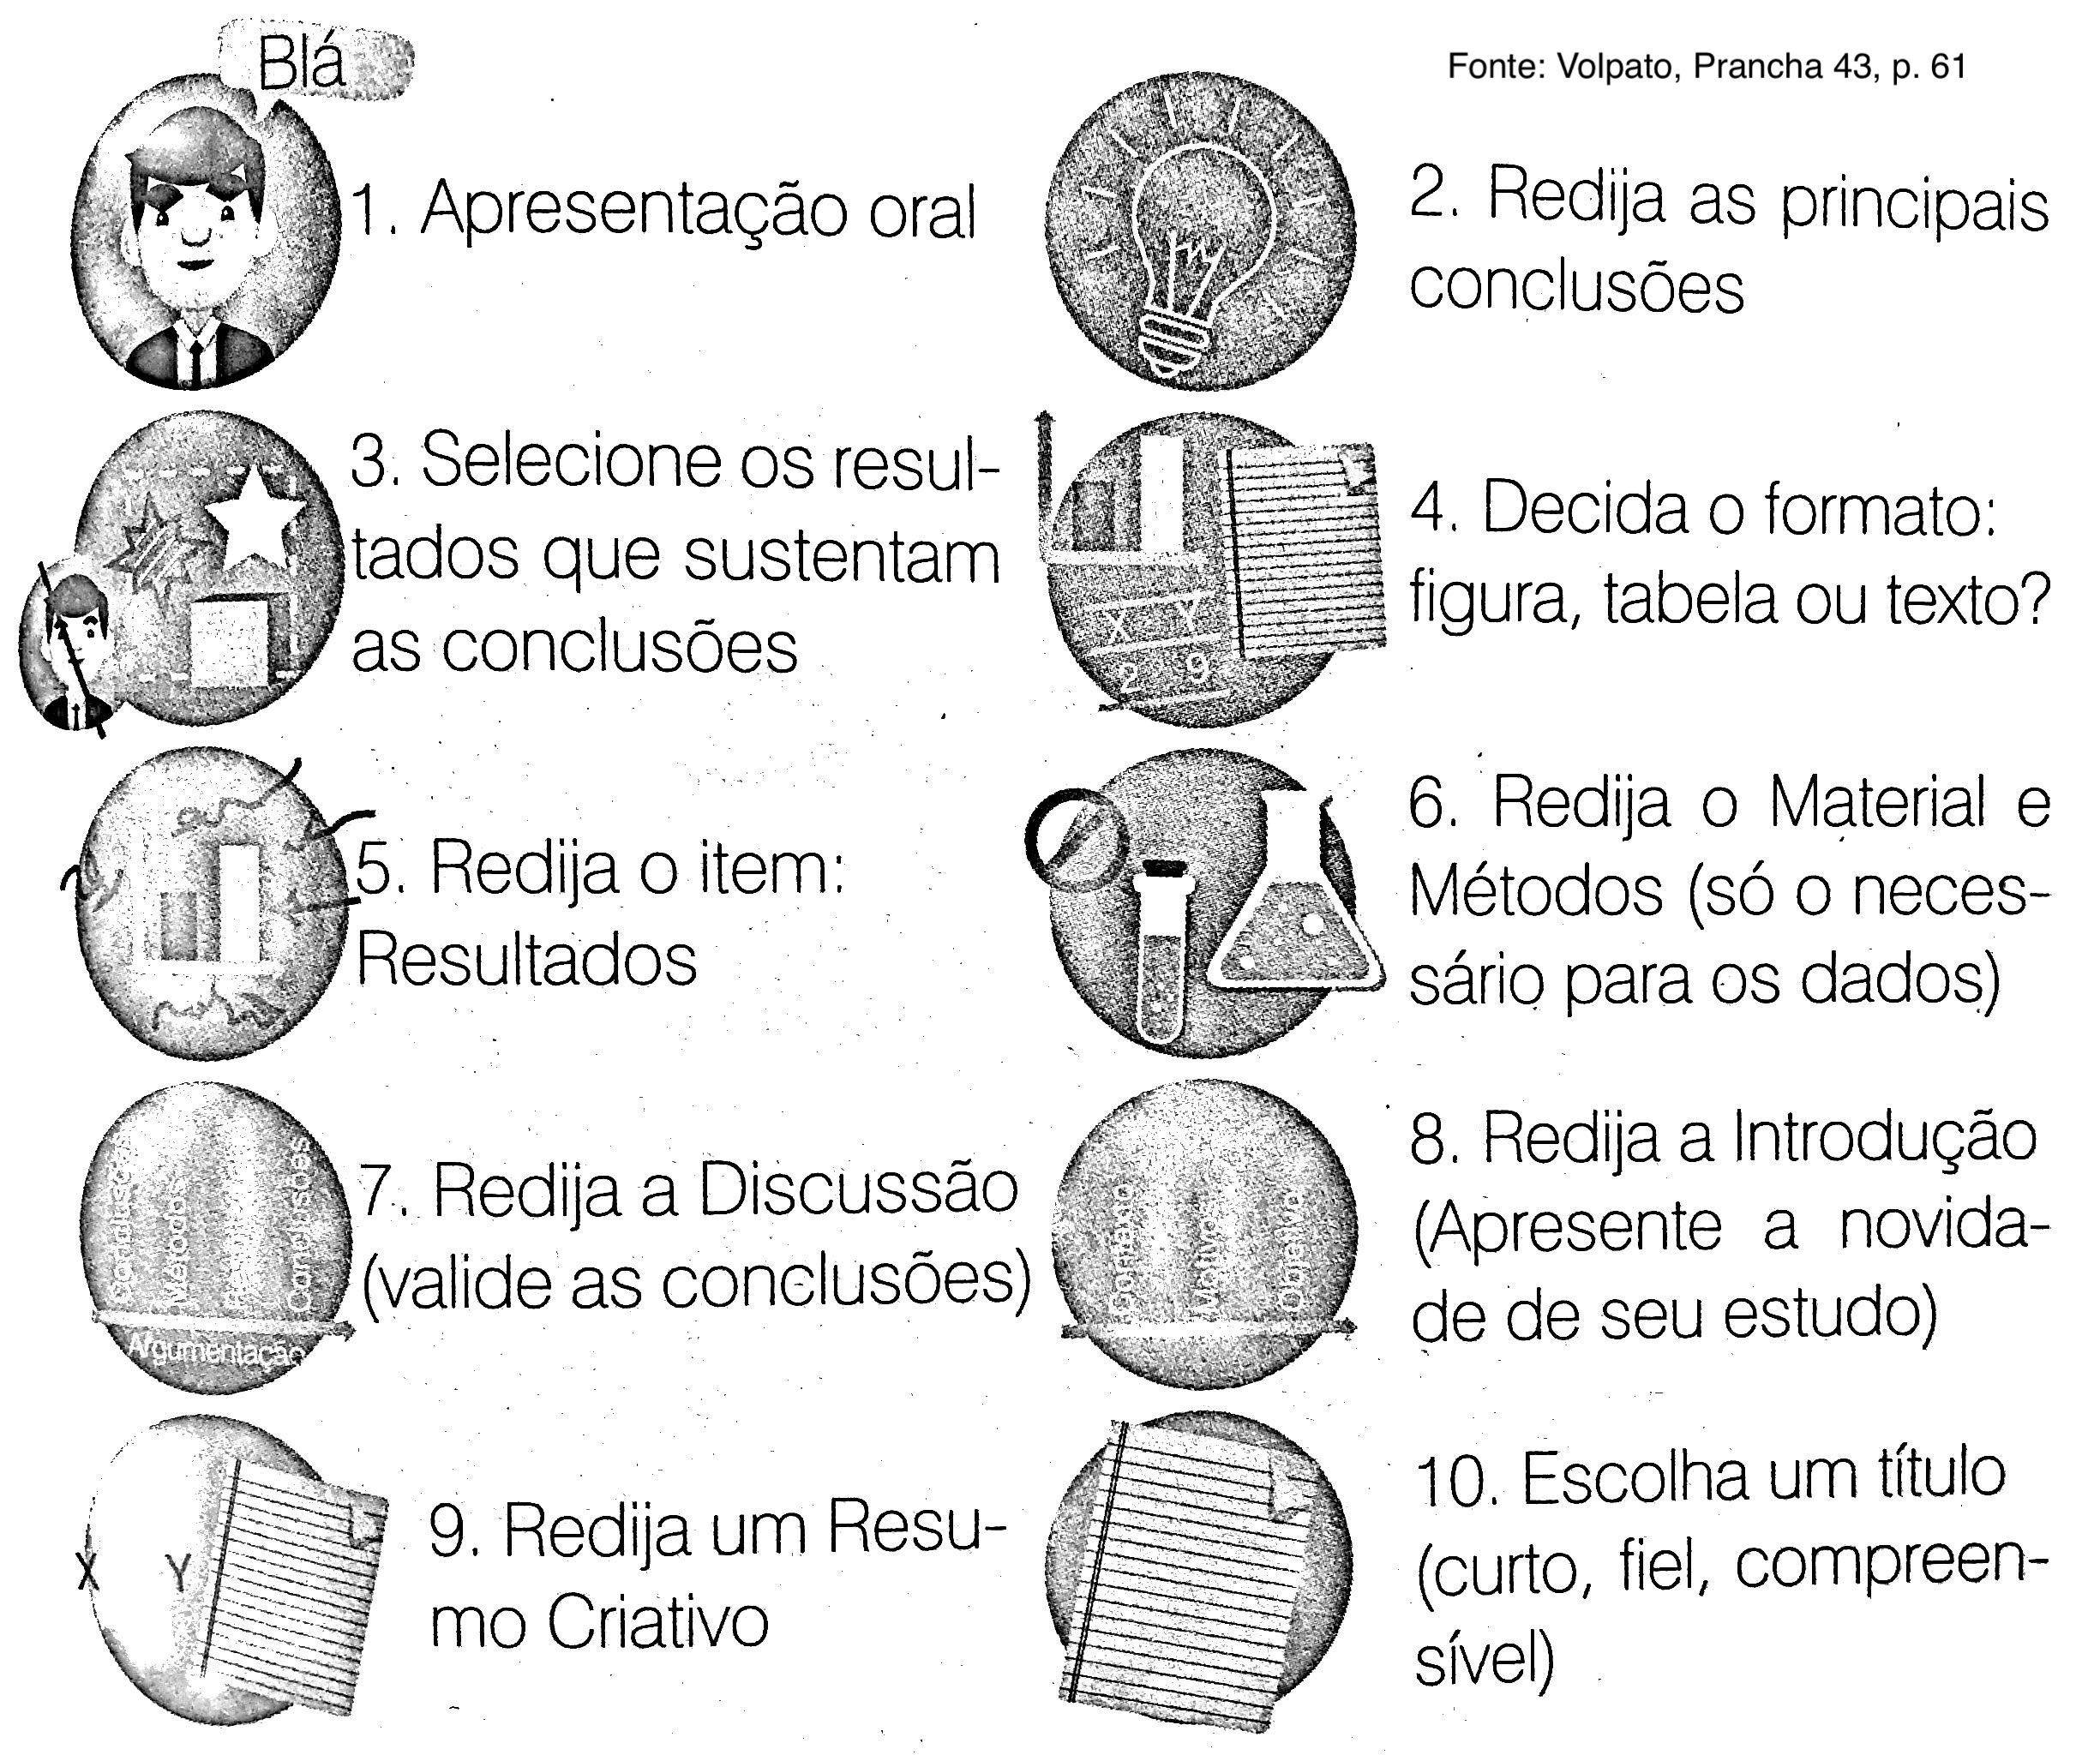
\includegraphics[scale=0.09]{figs/05/sequencia-redacao}
\caption{Sequencia de redação de artigo. Fonte: Volpato, 2017.}
\end{figure}
\end{frame}

\subsection*{Os 4 ``P''s}

%%
\begin{frame}{Os 4 ``Ps'' da confecção do artigo}
\begin{figure}
\centering
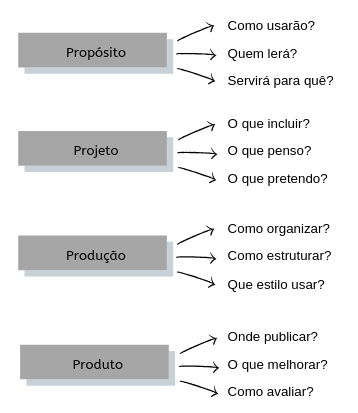
\includegraphics[scale=0.65]{figs/05/4ps}
\caption{Fonte: autor.}
\end{figure}
\end{frame}

%%
\begin{frame}
\begin{block}{\emph{``Scientific paper as a product''}}
\emph{``In spite of the importance of getting papers published as the main indicator of the scientists performance, students rarely get training in scientific writing. The basic features of a paper are  by intuition, which may be ineffective and/or inefficient. As a result misconceptions appear, leading to papers that are poorly structured and lacking clear focus.'' (Oliveira Jr. et al., 2006)}
\end{block}
\end{frame}

%%
\begin{frame}{Propósito}
\begin{itemize}
\item Entenda o público que quer atingir? 
\item Decida sobre comprimento, nível de detalhe e estilo 
\item Em geral, artigos serão lidos por revisores e por um público ``esperto'' e bem informado
\item Reduza margens de falha e avalie as condições
\end{itemize}
\end{frame}

%%
\begin{frame}{Projeto}
\begin{itemize}
\item Construa uma folha de conceito
\item Estruture seu pensamento 
\item Pense horizontal e verticalmente
\item Rascunhe figuras, gráficos, tabelas 
\item Idealize
\end{itemize}
\end{frame}


%%
\begin{frame}{Folha de conceito ``didática''}
\begin{figure}
\centering
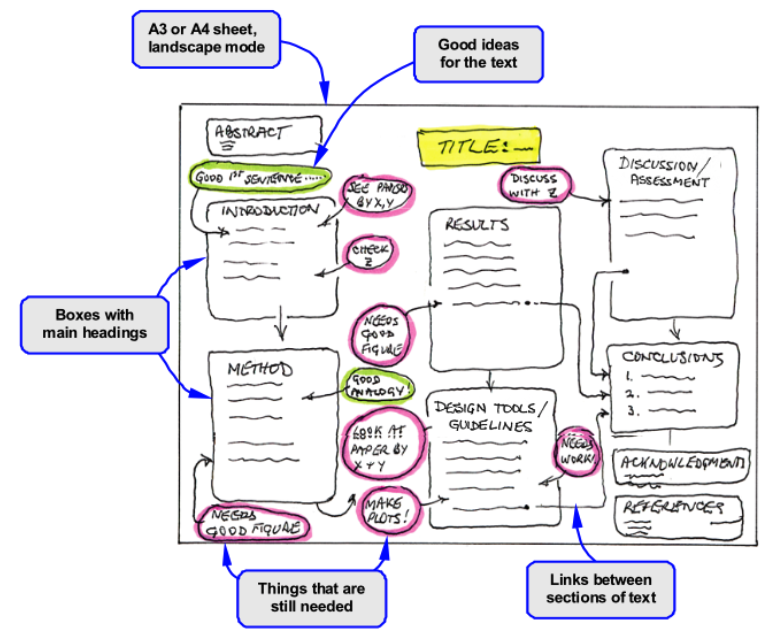
\includegraphics[scale=0.3]{figs/05/concept1}
\caption{Fonte: Ashby, 2005.}
\end{figure}
\end{frame}


%%
\begin{frame}{Folha de conceito ``didática'' expandida}
\begin{figure}
\centering
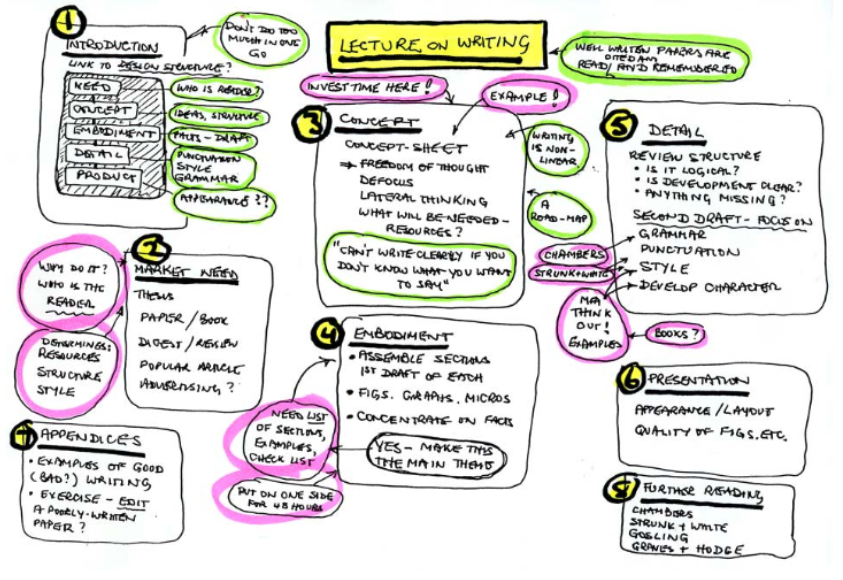
\includegraphics[scale=0.32]{figs/05/concept2}
\caption{Fonte: Ashby, 2005.}
\end{figure}
\end{frame}

%%
\begin{frame}{Produção}
\begin{itemize}
\item Fase mais difícil
\item Defina o título, o resumo, os métodos, os resultados 
\item Encontre as conclusões mais relevantes
\item Formate, estilize, decore e faça o polimento
\end{itemize}
\end{frame}


%%
\begin{frame}{Produto}
\begin{itemize}
\item Encontre o periódico mais adequado para publicar
\item Submeta e aguarde resposta
\item Ache o caminho do sucesso
\item Pense no futuro da pesquisa
\end{itemize}
\end{frame}

\section{O método IMRaD}

\begin{frame}{IMRaD (IMRD)}
\begin{itemize}
\item Acrônimo para: \textbf{I}ntrodução, \textbf{M}étodos, \textbf{R}esultados e \textbf{D}iscussão
\item São as componentes principais de um artigo
\item Às vezes, \textbf{M}ateriais e Métodos
\item Método mais comumente empregado
\item Atribuído a Louis Pasteur (1876) 
\item Adotado por periódicos científicos na década de 1940 (Wu, 2011)
\item Padronizado a partir da década de 1970 (ANSI Z39.16-1972)
\end{itemize}
\end{frame}

\begin{frame}{Opiniões...}
\begin{block}
\scriptsize{\emph{It is true that IMRAD does not always represent the order of actual research activities, but that alone does not make the scientific paper fraudulent. While IMRAD seems reflective of the currently dominant view of what is scientific, the format of the scientific paper may be influenced increasingly by technological advances in information processing and publishing as well as the pace of knowledge production. For now, IMRAD still rules, and modifications will continue.} (Wu, 2011)}
\end{block}
\end{frame}

\begin{frame}{Anatomia de um \textit{paper}}
\begin{figure}
\centering
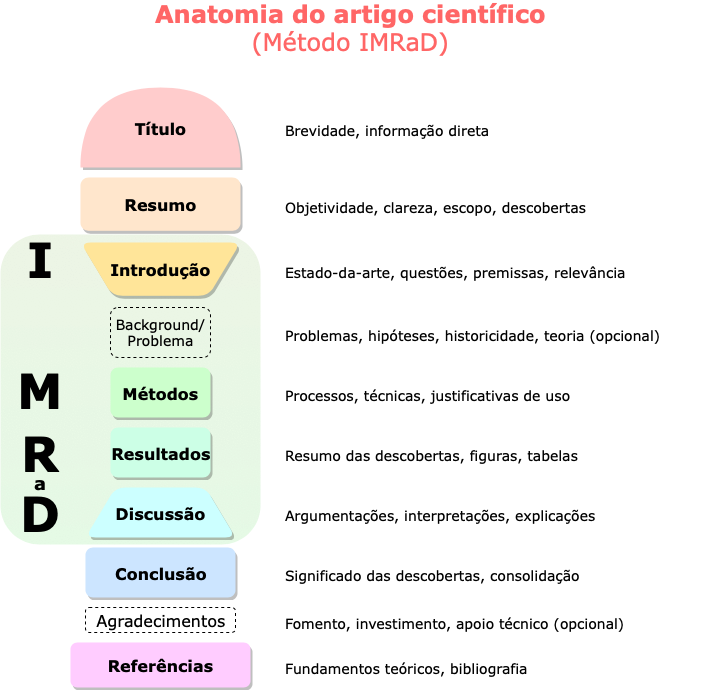
\includegraphics[scale=0.28]{figs/05/artigo-imrad}
\caption{\scriptsize{Fonte: Autor.}}
\end{figure}
\end{frame}

\begin{frame}{Tipos de artigos científicos}
\begin{itemize}
\item Revisões (\emph{Reviews})
\item Regulares (\emph{Regular paper})
\item Comunicações (\emph{Short Communication})
\end{itemize}
\end{frame}

\subsection{Anatomia do texto}

\begin{frame}{Escopo e organização das ideias}
\begin{itemize}
\item Defina seu escopo de ideias (do amplo ao específico)
\item Esboce parágrafos a partir das informações básicas
\item Construa parágrafos a partir de um \textit{tópico frasal}(\textit{topic sentence})
\item Agregue frases ao tópico frasal (nunca redija parágrafos de frase única!)
\end{itemize}
\end{frame}

\begin{frame}{Anatomia do parágrafo}
\begin{figure}
\centering
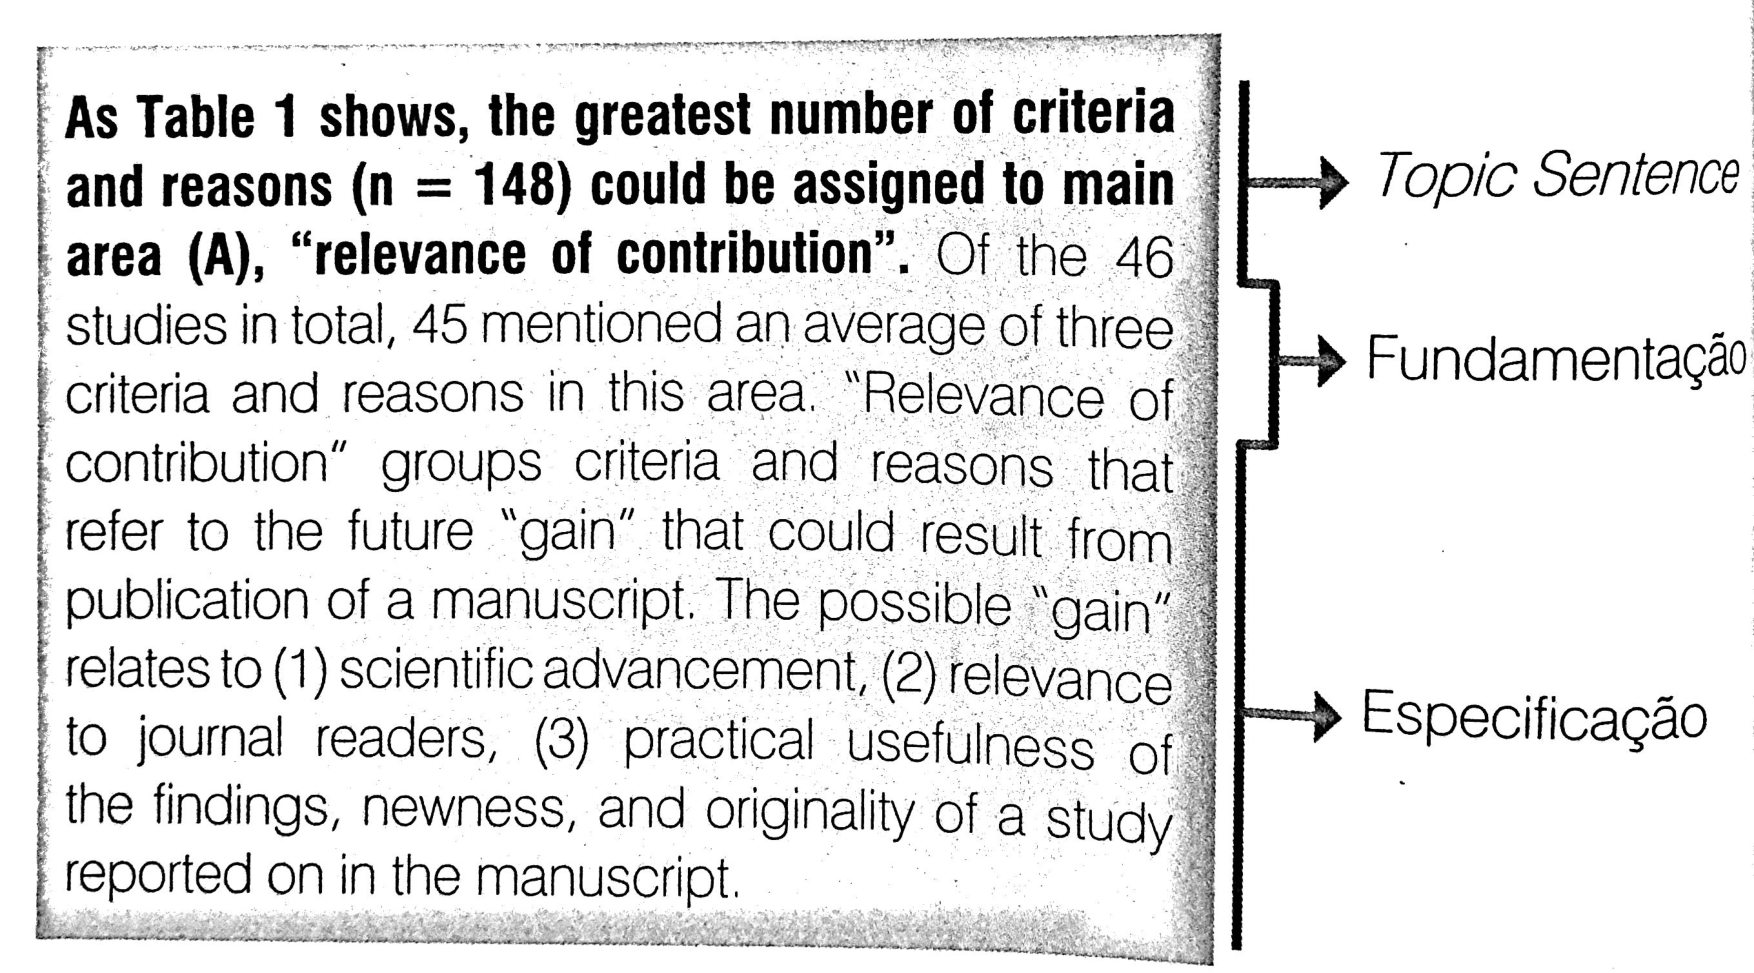
\includegraphics[scale=0.35]{figs/05/anatomia-paragrafo}
\caption{Anatomia do parágrafo. Fonte: Volpato, 2017.}
\end{figure}
\end{frame}

\begin{frame}{Cadência das ideias: estratégia ``e daí?''}
\begin{itemize}
\item O ``e daí?'' ajuda a conectar frases logicamente
\item Cada ``e daí"?'' termina uma frase e a resposta vem logo em seguida
\item O texto torna-se fluido
\item Conectivos são bons, mas, usados em excesso, ruins
\end{itemize}
\end{frame}

\begin{frame}
\begin{figure}
\centering
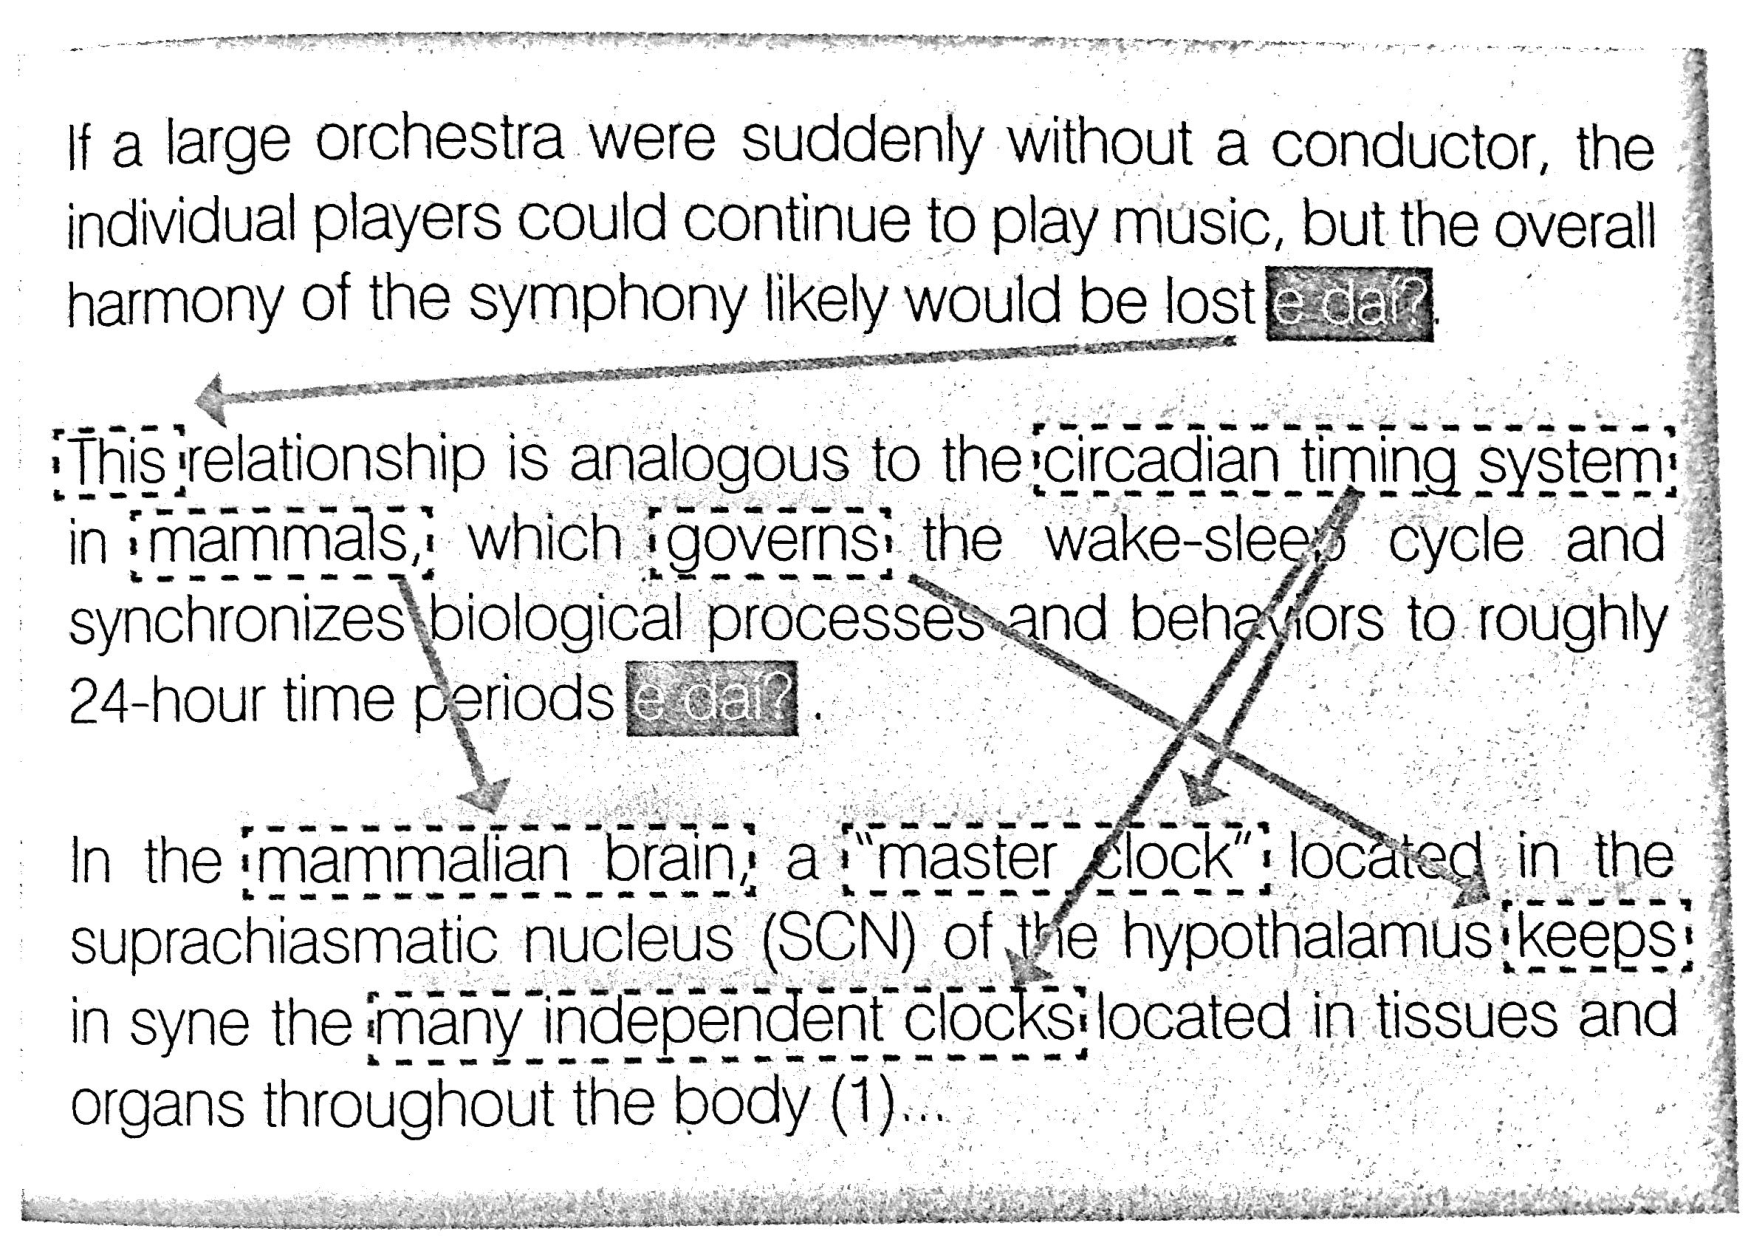
\includegraphics[scale=0.35]{figs/05/edai}
\caption{Estratégia do ``e daí?''. Fonte: Volpato, 2017.}
\end{figure}
\end{frame}

\begin{frame}{Metodologia AMADEUS} 
\begin{block}
\small{\emph{``In spite of the importance of getting papers published as the main indicator of the scientists' performance, students rarely get training in scientific writing. The basic features of a paper are learnt by intuition, which may be ineffective and/or inefficient. As a result misconceptions appear, leading to papers that are poorly structured and lacking clear focus. (Oliveira Jr. et al., 2006)''}}
\end{block}
\begin{itemize}
\item Escrita científica para não-nativos em inglês 
\item Veja o guia de 9 passos em (Oliveira Jr. et al., 2006)
\end{itemize}
\end{frame}

%%
\subsection{Declaração de objetivos}

\begin{frame}{Lógica nos objetivos}
\begin{itemize}
\item Enxergue objetivos como ``ideias que guiam ações'', não como ações declaradas 
\item Ex.: analisar/avaliar/investigar a condutividade térmica de materiais compósitos aquecidos acima de 200K 
\item Ex.: analisar se alterações da condutividade térmica em materiais compósitos aquecidos acima de 200K são  acentuadas por microfaturas paralelas ou normais ao fluxo de calor
\item Um paper baseia-se na formulação de novos métodos ou testes de hipóteses bem fundamentadas
\end{itemize}
\end{frame}

%%
\begin{frame}{Objetivo geral}
\begin{itemize}
\item A má declaração de objetivos é uma grande causa da sensação de ``estar perdido'' na pós 
\item A construção do ``onde se quer chegar'' pressupõe um entendimento claro do ``que se quer fazer''
\item Ex. OG: ``Testar se a insônia prejudica o desempenho escolar''
\end{itemize}
\end{frame}

\begin{frame}{Objetivos específicos}
\begin{itemize}
\item Insônia relaciona-se com ``horas dormidas/vezes em que se acorda''
\item Desempenho escolar relaciona-se com ``nota nas provas/assiduidade''
\item A partir disso, pode-se construir especificidades: 
\item OE1: ``Testar se há associação positiva entre tempo dormido e notas''
\item OE2: ``Avaliar se há associação positiva entre horas dormidas e assiduidade''
\end{itemize}
\end{frame}

\section{\emph{Plain English}}

\begin{frame}{Inglês na PG\footnote{Os dados a seguir foram extraídos de (Dantas-Lunn, 2018)}}
\begin{figure}
\centering
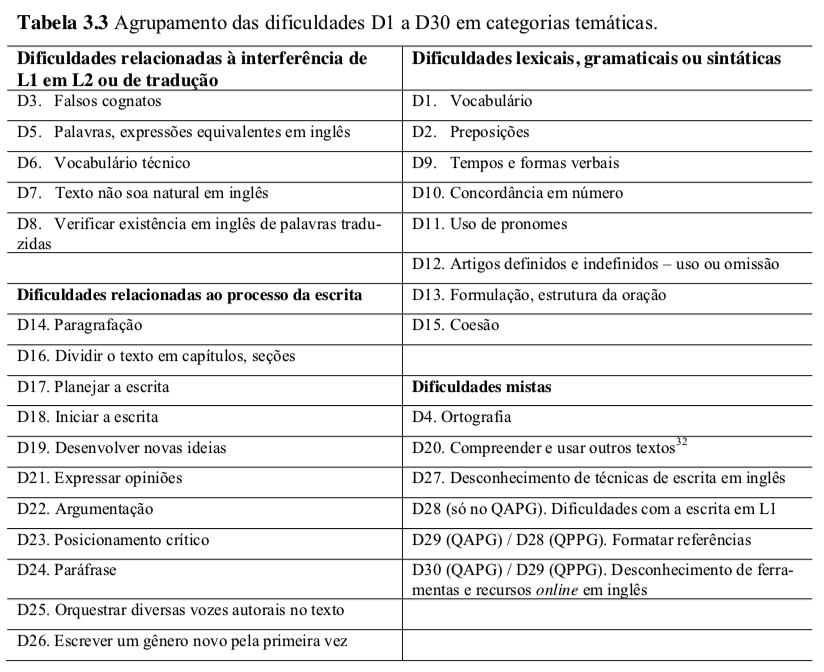
\includegraphics[scale=0.3]{figs/05/dificuldades-apg}
\end{figure}
\end{frame}

\begin{frame}
\begin{figure}
\centering
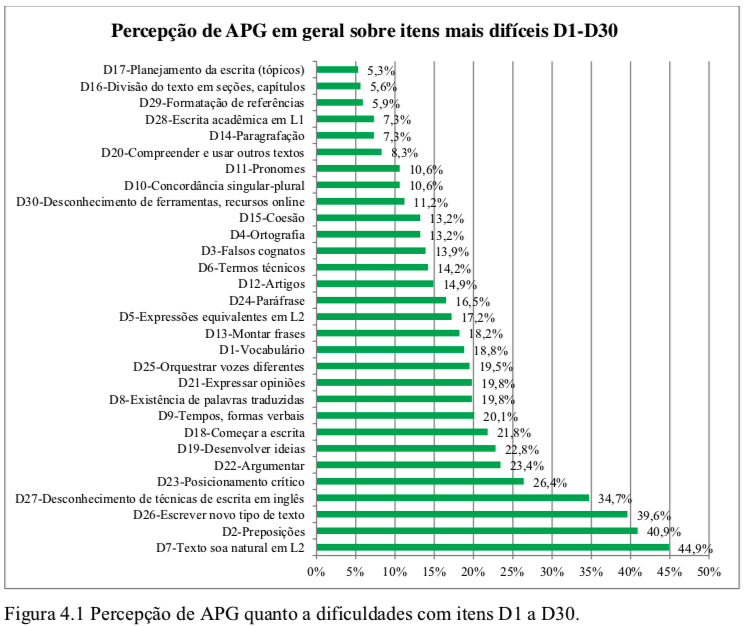
\includegraphics[scale=0.4]{figs/05/dificuldades-apg2}
\end{figure}
\end{frame}

\begin{frame}
\begin{block}{Dificuldade preponderante\footnote{Pesquisa realizada em PPGs da USP. Vide referência.}}
\small{\emph{Em primeiro lugar, \textbf{escrever um texto que ``soasse natural'' em inglês (D7)} foi percebido como difícil por 44,9\% dos alunos de pós-graduação. É uma dificuldade ligada à interferência do português (L1) na escrita em inglês (L2). Ao atribuírem tanta importância ao ``soar natural'' de seus textos em inglês, os pós-graduandos parecem ter a percepção de que faltaria algo em sua escrita em inglês, algo semelhante ao ``sotaque brasileiro'' na fala em inglês de um aprendiz, e essa falta/ausência seria um indício da suposta qualidade inferior de sua escrita.} (Dantas-Lunn, 2018)}
\end{block}
\end{frame}

\begin{frame}{O \emph{Plain English}\footnote{Baseado em: \url{https://posgraduando.com/plain-english/}}}
\begin{itemize}
\item A técnica do \emph{plain english} (inglês simples) significa reduzir a informação para facilitar o entendimento do leitor
\item \textit{Keep your sentences short!}
\end{itemize}
\end{frame}

\begin{frame}{Prática do \emph{plain english}: exemplo}
\begin{itemize}
\item Parágrafo em Português \\
>> \textit{A determinação de propriedades mecânicas de ligas metálicas contendo manganês foi realizada com o uso de testes de curva de tensão-deformação}
\item Traduação direta para o Inglês  \\
>> \textit{The determination of the mechanical properties of alloys containing manganese was carried out using the stress-strain tests}
\item Simplificando mais ainda  \\
>> \textit{Mechanical properties of alloys containing manganese were evaluated using the stress-strain tests}
\end{itemize}
\end{frame}

\begin{frame}
\begin{itemize}
\item Simplificando a linguagem \\
>> \textit{Mechanical properties of Mn-containing alloys were evaluated via stress-strain analyses}
\item Traduação direta para o Inglês  \\
>> \textit{Manganese alloys mechanical properties were evaluated by stress-strain analyses}
\end{itemize}
\end{frame}

\section{Organização do paper}

\subsection{Título, autores e afiliação}

\begin{frame}{Título (\emph{Title})\footnote{Baseado em (Zucolotto, 2011) e (Aquino, 2010) }}
\begin{itemize}
\item Um bom título descreve os conteúdos do artigo
\item \textbf{Função}: atrair a atenção do leitor
\end{itemize}
\end{frame}

\begin{frame}{Exemplo}
Artigo que reporta a influência do peso molecular sobre as propriedades mecânicas de fibras de Polianilina

\begin{block}{Título empobrecido e muito genérico}
\emph{Mechanical properties of Polyaniline fibers}
\end{block}
\end{frame}

\begin{frame}
\begin{block}{Expressa a ideia principal do trabalho, o tipo do filme e sua técnica de fabricação}
\emph{The influence of the MW on the mechanical properties of polyaniline electrospun fibers}

Palavras-chave: \emph{mechanical properties}, \emph{polyaniline}, \emph{electrospun fibers}
\end{block}
\end{frame}

%%
\begin{frame}{Palavras-chave}
\begin{itemize}
\item Palavras-chave (\emph{Keyword}): palavras fortemente associadas aos resultados do artigo
\item Em geral, no mínimo 3 a, no máximo, 6 palavras 
\item Evitar palavras presentes no título (inclua-as ) 
\end{itemize}
\end{frame}

%%
\begin{frame}{Autores}
\begin{itemize}
\item Os autores de um artigo \textbf{devem ser} capazes de apresentar, discutir e defender o artigo
\item Sequencia: autor principal, autores intermediários (contribuintes), último autor (sênior/líder de pesquisa)
\end{itemize}
\end{frame}

%% 
\begin{frame}{Notas sobre autoria}
\begin{itemize}
\item Autores são os que contribuem efetivamente
\item ``Premiação dos não comparecentes''
\item Evite ``caronagem''\footnote{Levar outrem na ``carona'' sob justificativa de estar ajudando.}
\item O nome dos autores deve seguir as normas do veículo de publicação
\item O papel de autor principal pode ser atrelado a casos especiais\footnote{coordenador de projeto; atrator de financiamento e fomento; orientador sênior; idealizador}
\end{itemize}
\end{frame}

\subsection{Afiliação}

%%
\begin{frame}{Ordem da informação}
\begin{block}{}
Grupo de pesquisa (ou laboratório), Departamento (ou Centro), Universidade (ou Instituição), Cidade, CEP, Caixa Postal (Zip Code, PO BOX), País.
\end{block}
\end{frame}

%%
\begin{frame}{Notas sobre afiliação}
\begin{itemize}
\item E-mail institucional é melhor visto do que nomes esdrúxulos \\ 
>> Ex. \textit{ze.solnascente@...}; \textit{teddybear54@...}; \textit{supergirl1995@...}
\item O autor principal ou correspondente, em geral, tem suas informações de contato no rodapé da primieira página
\end{itemize}

\end{frame}

%% === REFS
\begin{frame}[allowframebreaks]
\frametitle{Referências}
\begin{thebibliography}{9}
\setbeamertemplate{bibliography item}[book]
%
\bibitem{elsevier}\textit{Duties of Authors, Editors, Reviewers, and Publisher}. Policies and Guidelines: Int. J. of Nursing Sciences, Elsevier. Disponível em: \url{https://bit.ly/2lA3ePq}.
%
\bibitem{hwang2013}Hwang, K. \textit{Appropriate Roles for the Subscriber, Publisher, Editor, Author, and Reviewer in the Archives of Plastic Surgery}, doi: 10.5999/aps.2013.40.6.663.
%
\bibitem{wu2011}Wu, J. \textit{Improving the writing of research papers:IMRAD and beyond}. doi: DOI 10.1007/s10980-011-9674-3.
%
\bibitem{ashby2005}Ashby, M. \textit{How to write a paper}. Engg. Dept., Univ. of Cambridge, 2005.
%
\bibitem{volpato2017}Volpato, G.L. \textit{Método Lógico para Redação Científica}. 2a. ed., Best Writing, 2017.
%
\bibitem{oliveirajr2006}Oliveira Jr., O. N., Zucolotto, V., Aluísio, S. M. \textit{Developing strategies to produce better scientific papers: a Recipe for non-native users of English}. arXiv preprint cs/0611013 (2006)
%
\bibitem{lunn2018}Dantas-Lunn, M. S. \textit{A escrita em inglês na pós-graduação: dificuldades, convergências e divergências nas percepções de discentes e docentes}. Dissertação de Mestrado. FFLCH/USP, 2018.
%
\bibitem{zuco2011}Zucolotto, V. \textit{Workshop de Capacitação em Escrita Científica}, Disponível em: \url{http://www.escritacientifica.sc.usp.br/escrita/cursos-escrita/}
%
\bibitem{aquino2010}Aquino, I. S. \textit{Como escrever artigos científicos: sem ``arrodeio'' e sem medo da ABNT}, Saraiva, 2010.
\end{thebibliography}
\end{frame}